\documentclass[]{article}
\usepackage{lmodern}
\usepackage{amssymb,amsmath}
\usepackage{ifxetex,ifluatex}
\usepackage{fixltx2e} % provides \textsubscript
\ifnum 0\ifxetex 1\fi\ifluatex 1\fi=0 % if pdftex
  \usepackage[T1]{fontenc}
  \usepackage[utf8]{inputenc}
\else % if luatex or xelatex
  \ifxetex
    \usepackage{mathspec}
    \usepackage{xltxtra,xunicode}
  \else
    \usepackage{fontspec}
  \fi
  \defaultfontfeatures{Mapping=tex-text,Scale=MatchLowercase}
  \newcommand{\euro}{€}
\fi
% use upquote if available, for straight quotes in verbatim environments
\IfFileExists{upquote.sty}{\usepackage{upquote}}{}
% use microtype if available
\IfFileExists{microtype.sty}{%
\usepackage{microtype}
\UseMicrotypeSet[protrusion]{basicmath} % disable protrusion for tt fonts
}{}
\usepackage[margin=1in]{geometry}
\usepackage{longtable,booktabs}
\usepackage{graphicx}
\makeatletter
\def\maxwidth{\ifdim\Gin@nat@width>\linewidth\linewidth\else\Gin@nat@width\fi}
\def\maxheight{\ifdim\Gin@nat@height>\textheight\textheight\else\Gin@nat@height\fi}
\makeatother
% Scale images if necessary, so that they will not overflow the page
% margins by default, and it is still possible to overwrite the defaults
% using explicit options in \includegraphics[width, height, ...]{}
\setkeys{Gin}{width=\maxwidth,height=\maxheight,keepaspectratio}
\ifxetex
  \usepackage[setpagesize=false, % page size defined by xetex
              unicode=false, % unicode breaks when used with xetex
              xetex]{hyperref}
\else
  \usepackage[unicode=true]{hyperref}
\fi
\hypersetup{breaklinks=true,
            bookmarks=true,
            pdfauthor={J.E. Turcotte},
            pdftitle={MPG Comparisons between Manual and Automatic Transmissions},
            colorlinks=true,
            citecolor=blue,
            urlcolor=blue,
            linkcolor=magenta,
            pdfborder={0 0 0}}
\urlstyle{same}  % don't use monospace font for urls
\setlength{\parindent}{0pt}
\setlength{\parskip}{6pt plus 2pt minus 1pt}
\setlength{\emergencystretch}{3em}  % prevent overfull lines
\setcounter{secnumdepth}{0}

%%% Use protect on footnotes to avoid problems with footnotes in titles
\let\rmarkdownfootnote\footnote%
\def\footnote{\protect\rmarkdownfootnote}

%%% Change title format to be more compact
\usepackage{titling}

% Create subtitle command for use in maketitle
\newcommand{\subtitle}[1]{
  \posttitle{
    \begin{center}\large#1\end{center}
    }
}

\setlength{\droptitle}{-2em}
  \title{MPG Comparisons between Manual and Automatic Transmissions}
  \pretitle{\vspace{\droptitle}\centering\huge}
  \posttitle{\par}
  \author{J.E. Turcotte}
  \preauthor{\centering\large\emph}
  \postauthor{\par}
  \predate{\centering\large\emph}
  \postdate{\par}
  \date{May 17, 2016}



\begin{document}

\maketitle


\subsection{Executive Summary}\label{executive-summary}

In this brief study, we must explore the effect that automatic versus
manual transmissions has over miles-per-gallon fuel efficiency among a
sample group of 1974 model automobiles. First we looked at the data
itself, in brief. This we followed up with a simple examination of miles
per gallon as predicted by transmission type, but included indicators
that suggested that the real factors might be elsewhere. Following this,
we fit a simple model and compare it to a multivariate model that
included measured for transmission type, holding cylinders, horsepower
and weight converted constant. For further illustration, we view each
regressor separately.

\subsection{Assumptions}\label{assumptions}

\begin{itemize}
\itemsep1pt\parskip0pt\parsep0pt
\item
  The field `qsec' (or, from a stop, how many seconds it took for the
  vehicle to reach a quarter mile's distance) is likely a function of
  the car's power; i.e., a result, like miles per gallon, of the
  vehicle's configuration rather than a potential confounding cause OF
  miles per gallon. For that reason, I'm excluding it in any modelling
  of miles per gallon per vehicle.
\item
  Given the yes-or-no nature of whether or not a car is manufactured
  with or without automatic transmission, this data has been
  categorized, so named within the data, and is likely to be modelled
  using binomial logistic regression.
\item
  This study assumes that the engine power of each given vehicle
  proportional to the vehicle's weight. Rather, that the mass of the
  vehicle requires a matching size engine, and that a bigger engine will
  also contribute to the weight of the vehicle. Thus, a
  disproportionately designed vehicle might show up as an outlier.
\end{itemize}

\subsection{Examining the Data}\label{examining-the-data}

Looking at \emph{Figure 1}, we get a very quick sense of what the data
that we ahve to work with looks like. Given that not all these columns
(already exlcuding `vs' and `qsec') are easily read or in quite the
right format, the first step I've taken here is to rename the columns
and change the transmission data to a named factor.

Following this, \emph{Figure 2} gives us a brief summarization of the
better-named data that remains, excluding a few extra columns for
brevity.

A very simple \emph{Figure 3} binomial logistic regression line drawn
purely comparing miles per gallon (MPG) to whether (1) or not (0) a car
had a manual transition, there does APPEAR to be a strong
differentiation, BUT\ldots{} we've yet to examine any other details of
these cars. Further, giving the data points characteristics (size in
tonnage and color, re: number of cylinders), the subpatterning suggests
that either or both are significant factors\ldots{} rather, that they
are consistent with the same curve that we might have assigned to choice
of transmission alone.

Comparing coefficients between a simple and strict linear regression, in
\emph{Figure 4} between Miles per Gallon (MPG) and whether or not any
given car is a manual transmission versus a wider net cast, in
\emph{Figure 5} with several other regressors (being manual
transmission, cylinders, horsepower, and tonnage (converted from the
original measure of half-tons)), it becomes rather apparent that the use
of transmission is not the prevailing factor. \newpage

\subsection{Hypthotheses (\(H_{0}\) v.
\(H_{a}\))}\label{hypthotheses-hux5f0-v.-hux5fa}

Given the linear regression:
\[Y = 1 + \beta^{tr}_{i}X_{i} + \beta^{cyl}_{i}X_{i} + \beta^{wt}_{i}X_{i} + \epsilon_{i}\]
\ldots{}This paper shall \textbf{assume} that the choice of transmission
is not a significantly deterministic factor in a vehicle's
miles-per-gallon. Rather, in \(H_{0}\), that
\(\beta^{tr} < \beta^{wt} + \beta^{cyl}\) rather than in \(H_{a}\) where
\(\beta^{tr} >= \beta^{wt} + \beta^{cyl}\).

\subsection{Conclusion}\label{conclusion}

Notice that when considering only the type of transmission, we appear to
gain about 7.25 miles per gallon by going with a manual, but when
regressing for number of cylinders, 0.75mpg is removed per cylinder
added there, along with an insignificant subtraction for horsepower, and
a huge dectractor of over 5.2 miles per gallon per added ton in weight,
leaving merely an approximate \textbf{1.48 miles per gallon difference}
for our choice in transmission, with a standard error nearly as large.

Isolating for transmission, number of cylinders, and overall vehicle
tonnage, we see in \emph{Figures 6, 7, and 8}, verification that the
positive slope toward a manual transmission is dwarved by the negative
slopes of the first and third most impactful regressors, being the
vehicle's weight in tons and the number of cylinders invovled.

Given our probability value of \textbf{\textasciitilde{}0.31}, having
regressed for the other equivalent significant factors, this study
\textbf{fails to reject the null hypothesis} that the choice of
transmission makes any more than than a slight difference in fuel
economy. Certainly nothing compared to the choice in vehicle weight.

\subsection{Caveat}\label{caveat}

While this study does appear to have suggested a small but otherwise
statistically insignificant increase to fuel efficiency between
automatic and manual transmissions, this is not reliable information
insofar as the data provides no single model of car with both
transmission types. In the mid-70s, perhaps, a model had a transmission
type, and not the choice in the matter that we have today, but because
we do not know if automatic transmissions are not \textbf{heavier} than
manual transmissions, it may well be that the possible weight lost in
choosing a manual transmission might be completely explained by the
regression in fuel economy given a vehicle's overall mass.

\subsection{Source}\label{source}

Henderson and Velleman (1981), \emph{Building multiple regression models
interactively}. Biometrics, 37, 391--411. \newpage

\subsection{Appendix}\label{appendix}

\subsubsection{Figure 1 - Some of the
data}\label{figure-1---some-of-the-data}

\begin{longtable}[c]{@{}cccccccccc@{}}
\toprule
\begin{minipage}[b]{0.22\columnwidth}\centering\strut
~
\strut\end{minipage} &
\begin{minipage}[b]{0.06\columnwidth}\centering\strut
mpg
\strut\end{minipage} &
\begin{minipage}[b]{0.06\columnwidth}\centering\strut
cyl
\strut\end{minipage} &
\begin{minipage}[b]{0.06\columnwidth}\centering\strut
disp
\strut\end{minipage} &
\begin{minipage}[b]{0.05\columnwidth}\centering\strut
hp
\strut\end{minipage} &
\begin{minipage}[b]{0.06\columnwidth}\centering\strut
drat
\strut\end{minipage} &
\begin{minipage}[b]{0.06\columnwidth}\centering\strut
wt
\strut\end{minipage} &
\begin{minipage}[b]{0.05\columnwidth}\centering\strut
am
\strut\end{minipage} &
\begin{minipage}[b]{0.06\columnwidth}\centering\strut
gear
\strut\end{minipage} &
\begin{minipage}[b]{0.06\columnwidth}\centering\strut
carb
\strut\end{minipage}\tabularnewline
\midrule
\endhead
\begin{minipage}[t]{0.22\columnwidth}\centering\strut
\textbf{Mazda RX4}
\strut\end{minipage} &
\begin{minipage}[t]{0.06\columnwidth}\centering\strut
21
\strut\end{minipage} &
\begin{minipage}[t]{0.06\columnwidth}\centering\strut
6
\strut\end{minipage} &
\begin{minipage}[t]{0.06\columnwidth}\centering\strut
160
\strut\end{minipage} &
\begin{minipage}[t]{0.05\columnwidth}\centering\strut
110
\strut\end{minipage} &
\begin{minipage}[t]{0.06\columnwidth}\centering\strut
3.9
\strut\end{minipage} &
\begin{minipage}[t]{0.06\columnwidth}\centering\strut
2.62
\strut\end{minipage} &
\begin{minipage}[t]{0.05\columnwidth}\centering\strut
1
\strut\end{minipage} &
\begin{minipage}[t]{0.06\columnwidth}\centering\strut
4
\strut\end{minipage} &
\begin{minipage}[t]{0.06\columnwidth}\centering\strut
4
\strut\end{minipage}\tabularnewline
\begin{minipage}[t]{0.22\columnwidth}\centering\strut
\textbf{Mazda RX4 Wag}
\strut\end{minipage} &
\begin{minipage}[t]{0.06\columnwidth}\centering\strut
21
\strut\end{minipage} &
\begin{minipage}[t]{0.06\columnwidth}\centering\strut
6
\strut\end{minipage} &
\begin{minipage}[t]{0.06\columnwidth}\centering\strut
160
\strut\end{minipage} &
\begin{minipage}[t]{0.05\columnwidth}\centering\strut
110
\strut\end{minipage} &
\begin{minipage}[t]{0.06\columnwidth}\centering\strut
3.9
\strut\end{minipage} &
\begin{minipage}[t]{0.06\columnwidth}\centering\strut
2.875
\strut\end{minipage} &
\begin{minipage}[t]{0.05\columnwidth}\centering\strut
1
\strut\end{minipage} &
\begin{minipage}[t]{0.06\columnwidth}\centering\strut
4
\strut\end{minipage} &
\begin{minipage}[t]{0.06\columnwidth}\centering\strut
4
\strut\end{minipage}\tabularnewline
\begin{minipage}[t]{0.22\columnwidth}\centering\strut
\textbf{Datsun 710}
\strut\end{minipage} &
\begin{minipage}[t]{0.06\columnwidth}\centering\strut
22.8
\strut\end{minipage} &
\begin{minipage}[t]{0.06\columnwidth}\centering\strut
4
\strut\end{minipage} &
\begin{minipage}[t]{0.06\columnwidth}\centering\strut
108
\strut\end{minipage} &
\begin{minipage}[t]{0.05\columnwidth}\centering\strut
93
\strut\end{minipage} &
\begin{minipage}[t]{0.06\columnwidth}\centering\strut
3.85
\strut\end{minipage} &
\begin{minipage}[t]{0.06\columnwidth}\centering\strut
2.32
\strut\end{minipage} &
\begin{minipage}[t]{0.05\columnwidth}\centering\strut
1
\strut\end{minipage} &
\begin{minipage}[t]{0.06\columnwidth}\centering\strut
4
\strut\end{minipage} &
\begin{minipage}[t]{0.06\columnwidth}\centering\strut
1
\strut\end{minipage}\tabularnewline
\begin{minipage}[t]{0.22\columnwidth}\centering\strut
\textbf{Hornet 4 Drive}
\strut\end{minipage} &
\begin{minipage}[t]{0.06\columnwidth}\centering\strut
21.4
\strut\end{minipage} &
\begin{minipage}[t]{0.06\columnwidth}\centering\strut
6
\strut\end{minipage} &
\begin{minipage}[t]{0.06\columnwidth}\centering\strut
258
\strut\end{minipage} &
\begin{minipage}[t]{0.05\columnwidth}\centering\strut
110
\strut\end{minipage} &
\begin{minipage}[t]{0.06\columnwidth}\centering\strut
3.08
\strut\end{minipage} &
\begin{minipage}[t]{0.06\columnwidth}\centering\strut
3.215
\strut\end{minipage} &
\begin{minipage}[t]{0.05\columnwidth}\centering\strut
0
\strut\end{minipage} &
\begin{minipage}[t]{0.06\columnwidth}\centering\strut
3
\strut\end{minipage} &
\begin{minipage}[t]{0.06\columnwidth}\centering\strut
1
\strut\end{minipage}\tabularnewline
\begin{minipage}[t]{0.22\columnwidth}\centering\strut
\textbf{Hornet Sportabout}
\strut\end{minipage} &
\begin{minipage}[t]{0.06\columnwidth}\centering\strut
18.7
\strut\end{minipage} &
\begin{minipage}[t]{0.06\columnwidth}\centering\strut
8
\strut\end{minipage} &
\begin{minipage}[t]{0.06\columnwidth}\centering\strut
360
\strut\end{minipage} &
\begin{minipage}[t]{0.05\columnwidth}\centering\strut
175
\strut\end{minipage} &
\begin{minipage}[t]{0.06\columnwidth}\centering\strut
3.15
\strut\end{minipage} &
\begin{minipage}[t]{0.06\columnwidth}\centering\strut
3.44
\strut\end{minipage} &
\begin{minipage}[t]{0.05\columnwidth}\centering\strut
0
\strut\end{minipage} &
\begin{minipage}[t]{0.06\columnwidth}\centering\strut
3
\strut\end{minipage} &
\begin{minipage}[t]{0.06\columnwidth}\centering\strut
2
\strut\end{minipage}\tabularnewline
\begin{minipage}[t]{0.22\columnwidth}\centering\strut
\textbf{Valiant}
\strut\end{minipage} &
\begin{minipage}[t]{0.06\columnwidth}\centering\strut
18.1
\strut\end{minipage} &
\begin{minipage}[t]{0.06\columnwidth}\centering\strut
6
\strut\end{minipage} &
\begin{minipage}[t]{0.06\columnwidth}\centering\strut
225
\strut\end{minipage} &
\begin{minipage}[t]{0.05\columnwidth}\centering\strut
105
\strut\end{minipage} &
\begin{minipage}[t]{0.06\columnwidth}\centering\strut
2.76
\strut\end{minipage} &
\begin{minipage}[t]{0.06\columnwidth}\centering\strut
3.46
\strut\end{minipage} &
\begin{minipage}[t]{0.05\columnwidth}\centering\strut
0
\strut\end{minipage} &
\begin{minipage}[t]{0.06\columnwidth}\centering\strut
3
\strut\end{minipage} &
\begin{minipage}[t]{0.06\columnwidth}\centering\strut
1
\strut\end{minipage}\tabularnewline
\bottomrule
\end{longtable}

\subsubsection{Figure 2 - Summary of data after
retitling}\label{figure-2---summary-of-data-after-retitling}

\begin{longtable}[c]{@{}ccccc@{}}
\toprule
\begin{minipage}[b]{0.17\columnwidth}\centering\strut
MPG
\strut\end{minipage} &
\begin{minipage}[b]{0.17\columnwidth}\centering\strut
cylinders
\strut\end{minipage} &
\begin{minipage}[b]{0.17\columnwidth}\centering\strut
horsepower
\strut\end{minipage} &
\begin{minipage}[b]{0.18\columnwidth}\centering\strut
tons
\strut\end{minipage} &
\begin{minipage}[b]{0.18\columnwidth}\centering\strut
manual
\strut\end{minipage}\tabularnewline
\midrule
\endhead
\begin{minipage}[t]{0.17\columnwidth}\centering\strut
Min. :10.40
\strut\end{minipage} &
\begin{minipage}[t]{0.17\columnwidth}\centering\strut
Min. :4.000
\strut\end{minipage} &
\begin{minipage}[t]{0.17\columnwidth}\centering\strut
Min. : 52.0
\strut\end{minipage} &
\begin{minipage}[t]{0.18\columnwidth}\centering\strut
Min. :0.7565
\strut\end{minipage} &
\begin{minipage}[t]{0.18\columnwidth}\centering\strut
Min. :0.0000
\strut\end{minipage}\tabularnewline
\begin{minipage}[t]{0.17\columnwidth}\centering\strut
1st Qu.:15.43
\strut\end{minipage} &
\begin{minipage}[t]{0.17\columnwidth}\centering\strut
1st Qu.:4.000
\strut\end{minipage} &
\begin{minipage}[t]{0.17\columnwidth}\centering\strut
1st Qu.: 96.5
\strut\end{minipage} &
\begin{minipage}[t]{0.18\columnwidth}\centering\strut
1st Qu.:1.2906
\strut\end{minipage} &
\begin{minipage}[t]{0.18\columnwidth}\centering\strut
1st Qu.:0.0000
\strut\end{minipage}\tabularnewline
\begin{minipage}[t]{0.17\columnwidth}\centering\strut
Median :19.20
\strut\end{minipage} &
\begin{minipage}[t]{0.17\columnwidth}\centering\strut
Median :6.000
\strut\end{minipage} &
\begin{minipage}[t]{0.17\columnwidth}\centering\strut
Median :123.0
\strut\end{minipage} &
\begin{minipage}[t]{0.18\columnwidth}\centering\strut
Median :1.6625
\strut\end{minipage} &
\begin{minipage}[t]{0.18\columnwidth}\centering\strut
Median :0.0000
\strut\end{minipage}\tabularnewline
\begin{minipage}[t]{0.17\columnwidth}\centering\strut
Mean :20.09
\strut\end{minipage} &
\begin{minipage}[t]{0.17\columnwidth}\centering\strut
Mean :6.188
\strut\end{minipage} &
\begin{minipage}[t]{0.17\columnwidth}\centering\strut
Mean :146.7
\strut\end{minipage} &
\begin{minipage}[t]{0.18\columnwidth}\centering\strut
Mean :1.6086
\strut\end{minipage} &
\begin{minipage}[t]{0.18\columnwidth}\centering\strut
Mean :0.4062
\strut\end{minipage}\tabularnewline
\begin{minipage}[t]{0.17\columnwidth}\centering\strut
3rd Qu.:22.80
\strut\end{minipage} &
\begin{minipage}[t]{0.17\columnwidth}\centering\strut
3rd Qu.:8.000
\strut\end{minipage} &
\begin{minipage}[t]{0.17\columnwidth}\centering\strut
3rd Qu.:180.0
\strut\end{minipage} &
\begin{minipage}[t]{0.18\columnwidth}\centering\strut
3rd Qu.:1.8050
\strut\end{minipage} &
\begin{minipage}[t]{0.18\columnwidth}\centering\strut
3rd Qu.:1.0000
\strut\end{minipage}\tabularnewline
\begin{minipage}[t]{0.17\columnwidth}\centering\strut
Max. :33.90
\strut\end{minipage} &
\begin{minipage}[t]{0.17\columnwidth}\centering\strut
Max. :8.000
\strut\end{minipage} &
\begin{minipage}[t]{0.17\columnwidth}\centering\strut
Max. :335.0
\strut\end{minipage} &
\begin{minipage}[t]{0.18\columnwidth}\centering\strut
Max. :2.7120
\strut\end{minipage} &
\begin{minipage}[t]{0.18\columnwidth}\centering\strut
Max. :1.0000
\strut\end{minipage}\tabularnewline
\bottomrule
\end{longtable}

\subsubsection{Figure 3 - A simple bionomial
regression}\label{figure-3---a-simple-bionomial-regression}

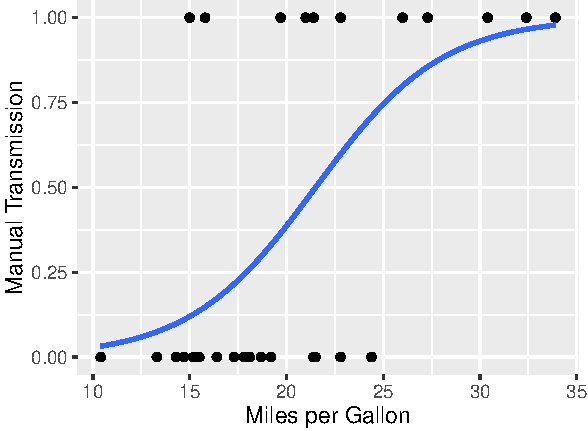
\includegraphics{study_files/figure-latex/simple binomial fit-1.pdf}
\newpage

\subsubsection{Figures 4 - Simple Linear
Model}\label{figures-4---simple-linear-model}

\begin{longtable}[c]{@{}ccccc@{}}
\toprule
\begin{minipage}[b]{0.21\columnwidth}\centering\strut
~
\strut\end{minipage} &
\begin{minipage}[b]{0.13\columnwidth}\centering\strut
Estimate
\strut\end{minipage} &
\begin{minipage}[b]{0.16\columnwidth}\centering\strut
Std. Error
\strut\end{minipage} &
\begin{minipage}[b]{0.12\columnwidth}\centering\strut
t value
\strut\end{minipage} &
\begin{minipage}[b]{0.12\columnwidth}\centering\strut
Pr(\textgreater{}\textbar{}t\textbar{})
\strut\end{minipage}\tabularnewline
\midrule
\endhead
\begin{minipage}[t]{0.21\columnwidth}\centering\strut
\textbf{(Intercept)}
\strut\end{minipage} &
\begin{minipage}[t]{0.13\columnwidth}\centering\strut
17.15
\strut\end{minipage} &
\begin{minipage}[t]{0.16\columnwidth}\centering\strut
1.125
\strut\end{minipage} &
\begin{minipage}[t]{0.12\columnwidth}\centering\strut
15.25
\strut\end{minipage} &
\begin{minipage}[t]{0.12\columnwidth}\centering\strut
1.134e-15
\strut\end{minipage}\tabularnewline
\begin{minipage}[t]{0.21\columnwidth}\centering\strut
\textbf{manual}
\strut\end{minipage} &
\begin{minipage}[t]{0.13\columnwidth}\centering\strut
7.245
\strut\end{minipage} &
\begin{minipage}[t]{0.16\columnwidth}\centering\strut
1.764
\strut\end{minipage} &
\begin{minipage}[t]{0.12\columnwidth}\centering\strut
4.106
\strut\end{minipage} &
\begin{minipage}[t]{0.12\columnwidth}\centering\strut
0.000285
\strut\end{minipage}\tabularnewline
\bottomrule
\end{longtable}

This regression suggests that your typical automatic will average about
17.15 miles per gallon, with your average manual transmission vehicle
will clock it at over 24 miles per gallon. But\ldots{}

\subsubsection{Figure 5 - Multivariate Linear
Model}\label{figure-5---multivariate-linear-model}

\begin{longtable}[c]{@{}ccccc@{}}
\toprule
\begin{minipage}[b]{0.32\columnwidth}\centering\strut
~
\strut\end{minipage} &
\begin{minipage}[b]{0.13\columnwidth}\centering\strut
Estimate
\strut\end{minipage} &
\begin{minipage}[b]{0.16\columnwidth}\centering\strut
Std. Error
\strut\end{minipage} &
\begin{minipage}[b]{0.12\columnwidth}\centering\strut
t value
\strut\end{minipage} &
\begin{minipage}[b]{0.12\columnwidth}\centering\strut
Pr(\textgreater{}\textbar{}t\textbar{})
\strut\end{minipage}\tabularnewline
\midrule
\endhead
\begin{minipage}[t]{0.32\columnwidth}\centering\strut
\textbf{(Intercept)}
\strut\end{minipage} &
\begin{minipage}[t]{0.13\columnwidth}\centering\strut
27.76
\strut\end{minipage} &
\begin{minipage}[t]{0.16\columnwidth}\centering\strut
2.723
\strut\end{minipage} &
\begin{minipage}[t]{0.12\columnwidth}\centering\strut
10.2
\strut\end{minipage} &
\begin{minipage}[t]{0.12\columnwidth}\centering\strut
9.364e-11
\strut\end{minipage}\tabularnewline
\begin{minipage}[t]{0.32\columnwidth}\centering\strut
\textbf{manual}
\strut\end{minipage} &
\begin{minipage}[t]{0.13\columnwidth}\centering\strut
1.478
\strut\end{minipage} &
\begin{minipage}[t]{0.16\columnwidth}\centering\strut
1.441
\strut\end{minipage} &
\begin{minipage}[t]{0.12\columnwidth}\centering\strut
1.026
\strut\end{minipage} &
\begin{minipage}[t]{0.12\columnwidth}\centering\strut
0.3142
\strut\end{minipage}\tabularnewline
\begin{minipage}[t]{0.32\columnwidth}\centering\strut
\textbf{cylinders}
\strut\end{minipage} &
\begin{minipage}[t]{0.13\columnwidth}\centering\strut
-0.7452
\strut\end{minipage} &
\begin{minipage}[t]{0.16\columnwidth}\centering\strut
0.5828
\strut\end{minipage} &
\begin{minipage}[t]{0.12\columnwidth}\centering\strut
-1.279
\strut\end{minipage} &
\begin{minipage}[t]{0.12\columnwidth}\centering\strut
0.2119
\strut\end{minipage}\tabularnewline
\begin{minipage}[t]{0.32\columnwidth}\centering\strut
\textbf{horsepower}
\strut\end{minipage} &
\begin{minipage}[t]{0.13\columnwidth}\centering\strut
-0.02495
\strut\end{minipage} &
\begin{minipage}[t]{0.16\columnwidth}\centering\strut
0.01365
\strut\end{minipage} &
\begin{minipage}[t]{0.12\columnwidth}\centering\strut
-1.828
\strut\end{minipage} &
\begin{minipage}[t]{0.12\columnwidth}\centering\strut
0.07855
\strut\end{minipage}\tabularnewline
\begin{minipage}[t]{0.32\columnwidth}\centering\strut
\textbf{I(tons - mean(tons))}
\strut\end{minipage} &
\begin{minipage}[t]{0.13\columnwidth}\centering\strut
-5.213
\strut\end{minipage} &
\begin{minipage}[t]{0.16\columnwidth}\centering\strut
1.84
\strut\end{minipage} &
\begin{minipage}[t]{0.12\columnwidth}\centering\strut
-2.834
\strut\end{minipage} &
\begin{minipage}[t]{0.12\columnwidth}\centering\strut
0.008603
\strut\end{minipage}\tabularnewline
\bottomrule
\end{longtable}

Instead, shifting our intercept to that of the average weight vehicle,
and regressive for cylinders, horsepower, and tonnage, we get a
completely different picture, showing that after other factors are
consider, very little detectable increase based on transmission alone
remains.

\subsubsection{Figures 6, 7, 8 - Individaulized Residual
Plots}\label{figures-6-7-8---individaulized-residual-plots}

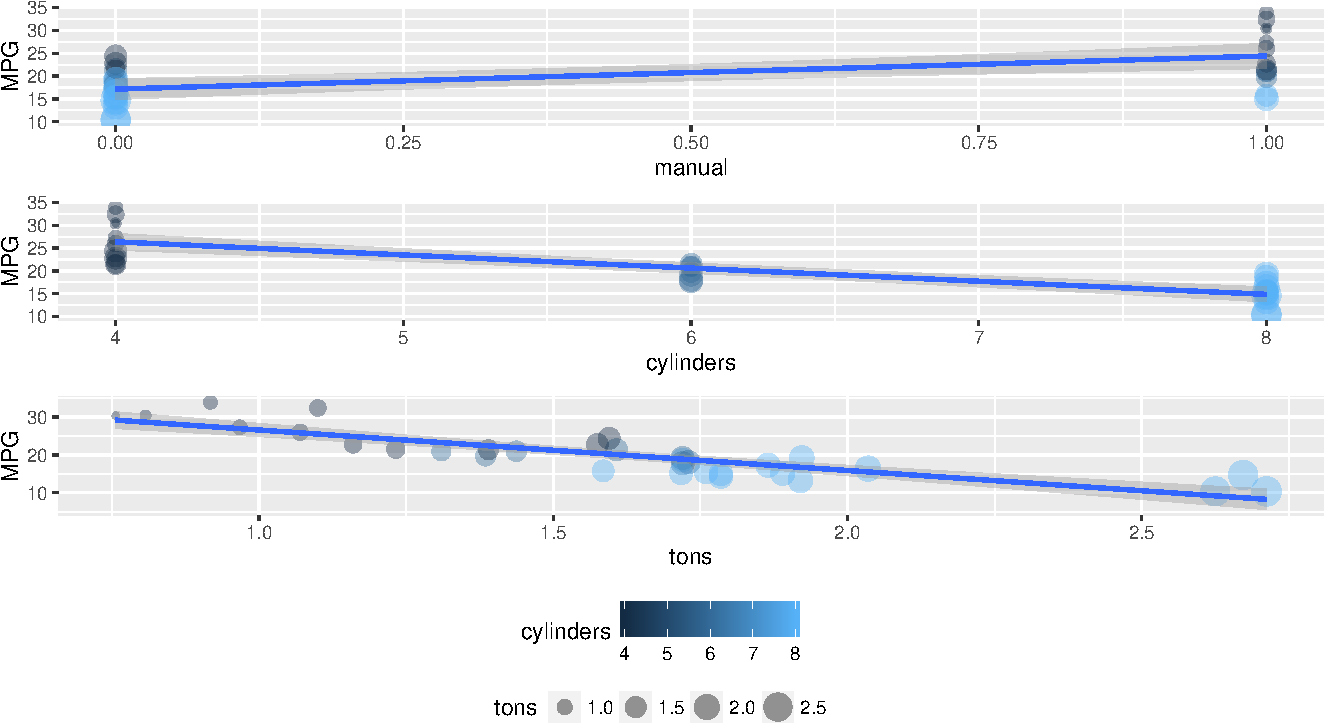
\includegraphics{study_files/figure-latex/plot the residuals of transmission-1.pdf}

\end{document}
